\center \textbf{CONVEXIDAD Y OPTIMIZACIÓN}
\center \textbf{\Large ENTREGA 1}
\center \textbf{ \textbf{Christian Limbert Paredes Aguilera}}

\line(1,0){400}

\footnote{
    Se llama \textbf{envoltura convexa} de $A$ al menor conjunto convexo que lo contiene o a la intersección de todos los convexos que contienen a $A$, denotado por $\co(A)$.
    También es equivalente a decir que
    $$\co(A)=\left\{\mbox{Combinación convexa de puntos de A.}\right\}$$
\label{uno}}

\footnote{
    Un conjunto $C\in \mathbb{R}^n$ se dice convexo cuando $C$ contiene las combinaciones convexas de sus puntos, si y sólo si
    $$\forall x_1,x_2\in C \Rightarrow \left[x_1,x_2\right]\subseteq C.$$
    Un conjunto es convexo si dados dos puntos el segmento que los une se queda adentro.
\label{dos}}

\footnote{
    Demostrar que la intersección de conjuntos convexos es convexo.\\\\
	Demostración.-\; Demostremos por contradicción. Sean $C_1$ y $C_2$ dos conjuntos convexos. Y sea 
	$$C=C_1\cap C_2.$$
	no convexo. Esto significa que existen $x$ e $y$ tales que 
	$$\left\{\lambda x + (1-\lambda)y:\lambda\in \mathbb{R}\right\}\not\subseteq C.$$ 
	Supongamos ahora que $x$ e $y$ están en $C$. Cómo ambos $C_1$ y $C_2$ son convexos, el segmento definido debe estar en ambos conjuntos. Es decir,
	$$\left\{\lambda x + (1-\lambda)y:\lambda\in \mathbb{R}\right\}\subseteq C.$$ 
	Lo que contradice nuestra suposición inicial. Por lo tanto, $C$ es convexo.
\label{tres}}

\begin{enumerate}[\bfseries \text{Ejercicio} 1.]

    \item \textbf{\boldmath Demuestra que la envoltura convexa de un conjunto $S\subset \mathbb{R}^n$ es la intersección de todos los conjuntos convexos de $\mathbb{R}^n$ que contienen a $S$.}

	\textbf{Demostración.-}\; Demostremos por contradicción. Supongamos que la envoltura convexa de un conjunto $S$, $\co(S)$ \footref{uno}, no es la intersección de todos los conjuntos convexos que contienen a $S$. Entonces, existe al menos un conjunto convexo, llámese $C$, que contiene a $S$ pero no contiene a $\co(S)$\footref{uno}. Es decir, existe un punto $p\in \co(S)$ tal que $p\notin C$.\\
	Por definición, $\co(S)$ es el conjunto de todas las combinaciones convexas de puntos en $S$. Por lo que el punto $p$ puede ser escrito como una combinación convexa de puntos en $S$. En otras palabras,
	$$p=\sum_{i=1}^k t_is_i\qquad s_i\in S,\; t_i\geq 0,\; \sum_{i=1}^k t_i=1.$$
	Dado que cada $s_i\in S$ y $S\subseteq C$. Entonces cada $s_1\in C$. Como $C$ es convexo y cada $s_i\in C$, la combinación convexa de los puntos $s_i$; es decir, el punto $p$, también debe estar en $C$. Lo que contradice nuestra suposición de que $p\notin C$. Por lo tanto, $\co(S)$ debe ser la intersección de todos los conjuntos convexos que contienen a $S$.
	\vspace{.5cm}

    \item \textbf{\boldmath La descripción de semiespacios de Voronoi: Sean $a$ y $b$ dos puntos distintos de $\mathbb{R}^n$. Demuestra que el conjunto de todos los puntos que están más cerca de $a$ (en la distancia Euclídea) que de $b$, i.e., $\left\{x\in \mathbb{R}^n : \|x-a\|_2 \leq \|x-b\|_2\right\}$, es un semiespacio. Descríbelo explícitamente como una desigualdad de la forma $c^T\cdot x \leq d$ (donde $c$ es un vector columna de $\mathbb{R}^n$). Haz una representación gráfica de la situación.}

	\textbf{Demostración.-}\; Podríamos 
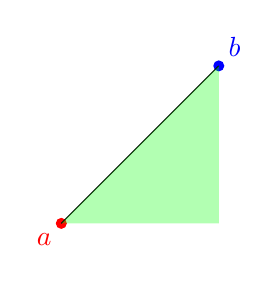
\begin{tikzpicture}
    % Define los puntos a y b
    \coordinate (a) at (0,0);
    \coordinate (b) at (2,2);
    
    % Dibuja los puntos a y b
    \fill[red] (a) circle (2pt) node[below left] {$a$};
    \fill[blue] (b) circle (2pt) node[above right] {$b$};
    
    % Dibuja la línea que separa el semiespacio
    \draw (a)--(b);
    
    % Dibuja el semiespacio
    \fill[green, opacity=0.3] (a)--(b)--(2,0)--cycle;
\end{tikzpicture}


    \item \textbf{\boldmath Demuestra que si $A$ y $B$ son conjuntos convexos de $\mathbb{R}^n$ entonces su intersección $A\cap B$ y su suma de Minkowsky $A+B$ son conjuntos convexos de $\mathbb{R}^n$.}

	\textbf{Demostración.-}\; Supongamos que $A$ y $B$ son conjuntos convexos en $\mathbb{R}^n$. Demostraremos que la intersección $A\cap B$ es convexa. Para ello, tomemos dos puntos cualesquiera $x,y\in A\cap B$. Dado que $x,y\in A$. Entonces, para todo $\lambda\in [0,1]$, se tiene:
	$$\lambda x+(1-\lambda)y\in A.$$
	De manera similar, dado que $x,y\in B$. Entonces, para todo $\lambda \in [0,1]$, también tenemos:
	$$\lambda x+(1-\lambda)y\in B.$$
	Por lo tanto, 
	$$\lambda x+(1-\lambda)y\in A\cap B,$$
	lo que implica que la intersección de conjuntos convexos es convexa.

	Para demostrar la suma de Minkowski. Sean $A$ y $B$ dos conjuntos convexos. Luego, consideremos dos puntos arbitrarios $x_1+x_2,y_1+y_2\in A+B$, donde $x_1,y_1\in A$ y $x_1,y_2\in B$. Como $A$ y $B$ son convexos, entonces para cualquier $\lambda$ tal que $0\leq \lambda \leq 1$, tenemos que 
	$$\lambda x_1+(1-\lambda)y_1\in A \quad \text{y}\quad \lambda x_2+(1-\lambda)y_2\in B.$$
	Por lo tanto,
	$$\lambda x_1+(1-\lambda)y_2+\lambda x_2+(1-\lambda)y_2= \lambda(x_1+x_2)+(1-\lambda)(y_1+y_2).$$
	está en $A+B$. Así, la suma de Minkowski de conjuntos convexos es convexa.
	
\end{enumerate}
